% Gantt simplificat (des. 2025 -- ago. 2026). Les pauses (març, juny) es veuen com a buits.
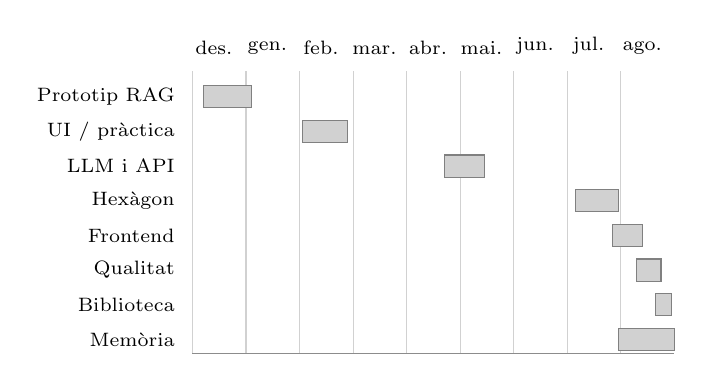
\begin{tikzpicture}[
  font=\scriptsize,
  x=0.68cm, y=0.44cm,
  bar/.style={fill=black!18, draw=black!50, thin},
]
\foreach \x/\m in {0/des.,1/gen.,2/feb.,3/mar.,4/abr.,5/mai.,6/jun.,7/jul.,8/ago.} {
  \node[anchor=south] at (3.3+\x+0.4, 8.45) {\m};
  \draw[black!18] (3.3+\x, 0.1) -- (3.3+\x, 8.25);
}
\draw[black!45] (3.3,0.1) -- (12.3,0.1);
\providecommand{\tfmganttbar}[4]{%
  \node[anchor=east, align=right] at (3.15,#1) {#4};
  \fill[bar] (3.3+#2,#1-0.32) rectangle (3.3+#3,#1+0.32);
}
\tfmganttbar{7.5}{0.2}{1.1}{Prototip RAG}
\tfmganttbar{6.5}{2.05}{2.9}{UI / pràctica}
\tfmganttbar{5.5}{4.7}{5.45}{LLM i API}
\tfmganttbar{4.5}{7.15}{7.95}{Hexàgon}
\tfmganttbar{3.5}{7.85}{8.4}{Frontend}
\tfmganttbar{2.5}{8.3}{8.75}{Qualitat}
\tfmganttbar{1.5}{8.65}{8.95}{Biblioteca}
\tfmganttbar{0.5}{7.95}{9.0}{Memòria}
\end{tikzpicture}
